\chapter{Trabalhos Relacionados}

No que diz respeito a interatividade entre usuários e ambientes virtuais ou jogos fisicamente interativos,
existem muitos trabalhos enfocados a segmentos de categorias específicas. Como comentado anteriormente
a maioria deles requer hardware especial, ambientes especiais ou recursos adicionais, para sua implementação.

\cite{DeteccaoInterface}, em seu trabalho de conclusão de curso, utilizam uma camera USB genérica para detectar
o olhos do usuário, depois de detectado o rosto e então transmitir a posição do usuário em relação a camera,
fazendo uma camera no ambiente virtual se movimentar também, desenvolveram então um ambiente virtual imersivo,
onde a maneira como o usuário visualizava o ambiente virtual dependia da posição de onde ele olhava para o monitor(figura \ref{DeteccaoInterface}).
O programa foi desenvolvido utilizando a linguagem C++, auxiliada das bibliotecas OpenCV, para processamento de imagem,
OpenGL, para desenho do ambiente virtual e newmat para cálculo de matrizes. Para detecção foi utilizado o método de
Viola e Jones, baseado em características do tipo Haar utilizando AdaBoost e filtro de Kalman para fazer a correção
e predição da posição da face na imagem. Como resultado o programa rodou a uma taxa de 25 quadros por segundo,
utilizando imagem com resolução 640 X 480 pixels.

\begin{figure}[h]
    \center
    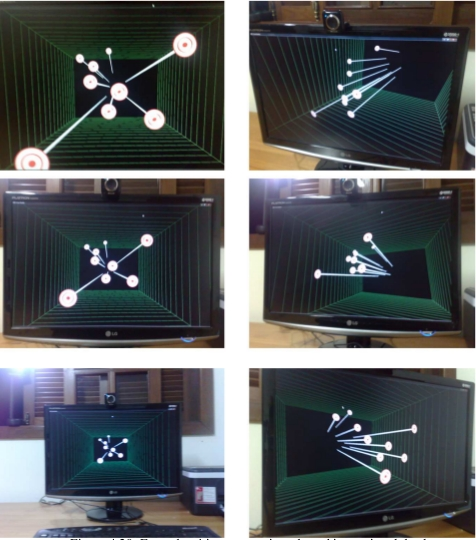
\includegraphics[scale=1.0]{imagens/DeteccaoInterface.jpg}

    \caption{Variação da perspectiva no ambiente virtual}
    \label{DeteccaoInterface}
\end{figure}

